% !TEX root = MusicFormatsMaintainanceGuide.tex

% -------------------------------------------------------------------------
\chapter{The generators}%%%JMI 'The' too much?
% -------------------------------------------------------------------------

A generator creates a music score ex-nihilo, without any description of the music being input. It's behaviour can be adapted to the users needs with options if needed.

Generators are supplied in the \generators\ directory. They don't have any interface in at the time of this writing, even though they could. %%%JMI

%%%JMI	musicformatsversion.cpp		keep this  sample?

% -------------------------------------------------------------------------
\section{{\tt MusicAndHarmonies}}
% -------------------------------------------------------------------------

\code{MusicAndHarmonies.cpp}%%% JMI


% -------------------------------------------------------------------------
\section{{\tt Mikrokosmos3Wandering}}
% -------------------------------------------------------------------------

This service produces the score for Zoltán Kodály's Mikrokosmos III Wandering score, taking inspiration from the same example in Abjad (\url{http://abjad.mbrsi.org/literature_examples/bartok.html}).
Is was written in the first place to check the MSR \API\ before writing the MSDL converter.

The score produced is shown at \figureRef{Zoltán Kodály's Mikrokosmos III Wandering}.
\begin{figure}[htbp]
\begin{center}
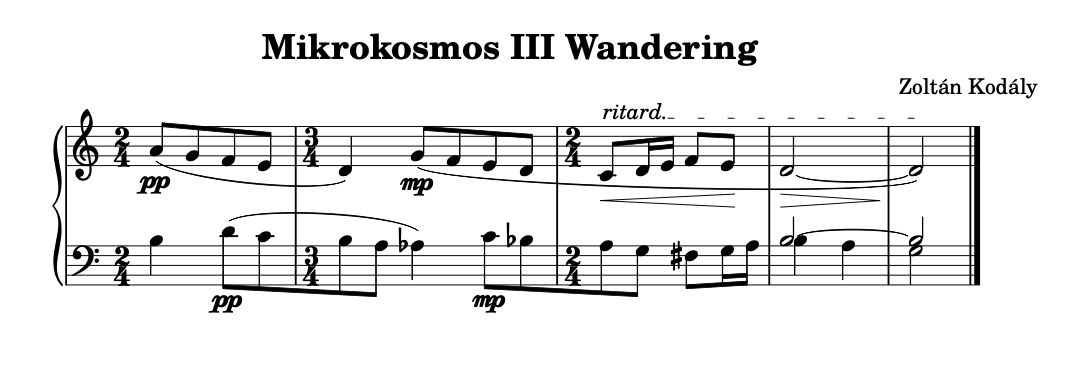
\includegraphics[scale=0.9]{../graphics/MikrokosmosIIIWandering.png}
\caption{Zoltán Kodály's Mikrokosmos III Wandering}
\label{Zoltán Kodály's Mikrokosmos III Wandering}
\end{center}
\end{figure}


% -------------------------------------------------------------------------
\section{{\tt LilyPondIssue34}}
% -------------------------------------------------------------------------

This service produces the same score as that obtained by:
\begin{lstlisting}[language=CPlusPlus]
xml2ly -auto-output-file-name gracenotes/LilyPondIssue34.xml
\end{lstlisting}

The resulting score is shown at \figureRef{The LilyPondIssue34 score}.
\begin{figure}[htbp]
\begin{center}
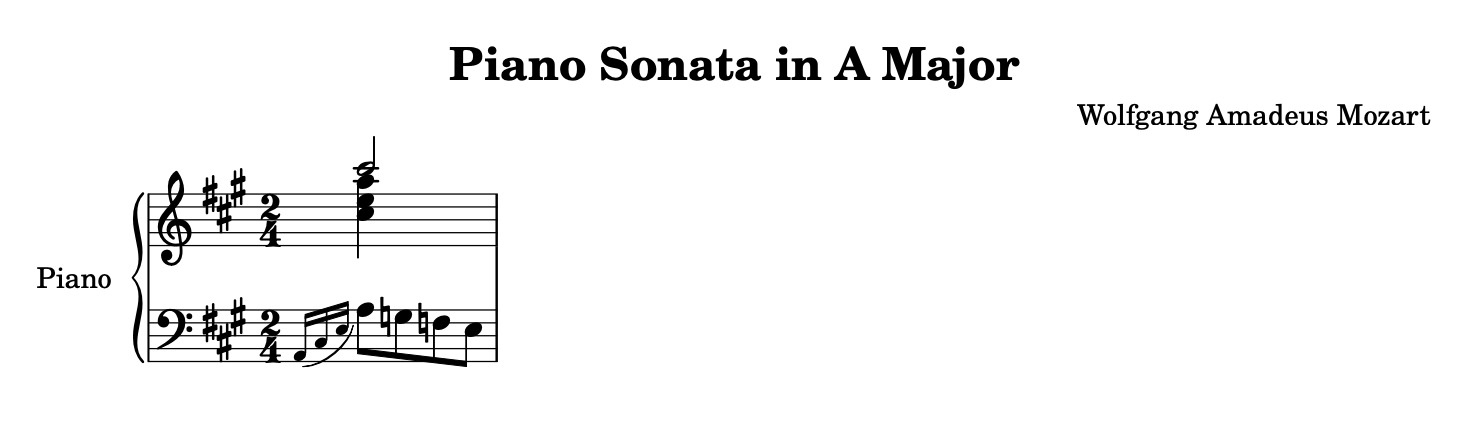
\includegraphics[scale=0.9]{../graphics/LilyPondIssue34.png}
\caption{The LilyPondIssue34 score}
\label{The LilyPondIssue34 score}
\end{center}
\end{figure}

The name \fileName{LilyPondIssue34} stems from the fact that translating this \mxml\ file to LilyPond\ with \fileName{\mxmlToLy} exhibits the famous \lily\ issue \#34.

This example was written to design a \lily-oriented interface to LPSR, preparing the grounds for \lily\ export to other formats. This work in in progress at the time of this writing.

